%
% Technical report RA-019/06 (DS)
%
\documentclass[a4paper,10pt,oneside,final]{dweiss-technote}

\usepackage[small]{titlesec}
\usepackage[UTF8]{inputenc}
\usepackage[OT4]{fontenc}
\usepackage[polish,english]{babel}
\usepackage{graphicx}
\usepackage[bookmarks=true,unicode, dvipdfm]{hyperref}
\usepackage{fancyvrb}
\usepackage[footnotesize, sc]{caption}
\usepackage[raggedright]{subfigure}
\setcaptionmargin{1cm}
\usepackage{url}\urlstyle{sf}
\usepackage{xcolor}
\usepackage{fancyhdr}
\usepackage{datetime}
\usepackage{setspace}
\usepackage[clock]{ifsym}
\usepackage{bbding}
\usepackage{tabularx}
\usepackage{booktabs}
\usepackage{varioref}

% utopia font set.
\usepackage{qtimes}


\definecolor{linkscolor}{rgb}{1,1,0}

\hypersetup{
  bookmarksopen=false,
  bookmarksopenlevel=3,
  bookmarksnumbered=true,
%  
  colorlinks=false,
  citebordercolor=0.64 0.68 0.86,
  filebordercolor=0.64 0.68 0.86,
  linkbordercolor=0.64 0.68 0.86,
  menubordercolor=0.64 0.68 0.86,
  pagebordercolor=0.64 0.68 0.86,
  urlbordercolor=0.64 0.68 0.86,
  runbordercolor=0.64 0.68 0.86,
%  
  pdfpagemode=UseOutlines,
  pdfstartview=Fit,
%
  pdftitle={},
  pdfauthor={Dawid Weiss},
  pdfkeywords={}
}	

\RecustomVerbatimEnvironment{Verbatim}{Verbatim}
  {fontsize=\footnotesize,rulecolor=\color{gray},
   % frame=leftline,framerule=2mm,framesep=5mm
   numbers=left}

\DefineVerbatimEnvironment{ShellVerbatim}{Verbatim}
  {fontsize=\footnotesize, numbers=left}

% \DeclareGraphicsExtensions{.eps}

\newcommand{\todo}[1]{\sidenote{{\color{red}TODO}}%
\medskip\noindent\fbox{\parbox{0.9\textwidth}{{\textit{\small#1}}}}}

\def\BibTeX{{\rm B\kern-.05em{\sc i\kern-.025em b}\kern-.08em
    T\kern-.1667em\lower.7ex\hbox{E}\kern-.125emX}}

\newenvironment{important}%
{\noindent\begin{flushright}\makebox[\width]{\Huge\HandRight}\hspace{0.5cm}\begin{minipage}[b]{0.8\textwidth}\ignorespaces\small}%
{\end{minipage}\end{flushright}\ignorespacesafterend} 
\newcommand{\fname}[1]{\texttt{#1}}

\newcommand{\smallurl}[1]{{\small\url{#1}}}

\newcommand{\tabcaption}[1]{\multicolumn{1}{c}{#1}}

\renewcommand{\textsc}[1]{{\scriptsize \MakeUppercase{#1}}}
\newcommand{\jme}{\textsc{j2me}}

\newcommand{\method}[1]{\textsc{#1}}
\newcommand{\class}[1]{\textsc{#1}}

\DefineVerbatimEnvironment{codeblock}{Verbatim}%
    {frame=lines,numbers=none,numbersep=0pt,fontsize=\scriptsize}

\pagestyle{cvsidstyle}

\date{}

\cvsid{$Id: j2me-testing.tex 2523 2006-12-20 13:01:14Z dweiss $}

\title{A Framework for Testing Mobile~Applications in~Java2~Microedition}

\author{%
\begin{tabular}{c c}
Dawid Weiss & Marcin Zduniak \\
\small\url{dawid.weiss@cs.put.poznan.pl} & \small\url{mzduniak@j2me.pl} \\
\small Poznan University of Technology & \small Poznan University of Technology \\
\end{tabular}}

\begin{document}

\maketitle
\thispagestyle{cvsidfirst}

\begin{center}
\fbox{\textsc{technical report number: \textbf{RA-019/06} (DS)}}
\end{center}

\vspace{3ex}
\begin{abstract}
Applications for mobile devices are becoming widespread. The more
complex they become, the more evident is the need for automated testing frameworks allowing
unsupervised regression tests, with particular focus on the graphical user interface. While
automated testing (also called \emph{capture-replay}) has been thoroughly discussed in literature
with respect to desktop applications, mobile development limits automation possibilities
significantly. To our best knowledge no comprehensive framework for automated testing of mobile
applications exists. In this paper we demonstrate preliminary results of our attempt to design and
implement a framework for capturing and replaying user interaction in Java2 Microedition
environment. The outcomes are so far very promising and have been evaluated on a complex commercial 
mobile navigation system.
\end{abstract}

\selectlanguage{polish}%
\begin{abstract}
Programy na urządzenia mobilne stają się coraz bardziej powszechne. Wraz ze wzrostem
możliwości obliczeniowych urządzeń, programy na nie pisane stają się coraz bardziej skomplikowane
i coraz bardziej pilna jest potrzeba pisania do nich różnego rodzaju testów, szczególnie uwzględniających
graficzny interfejs użytkownika (GUI). Znane ze środowiska aplikacji desktopowych testy typu
nagraj-odtwórz (ang.~\emph{capture-replay}) są właściwie nieistniejące w świecie aplikacji na urządzenia
mobilne w wyniku utrudnień i ograniczeń narzucanych przez to środowisko. W niniejszym raporcie zaprezentowano
wyniki badań dotyczących próby zbudowania programu do testowania automatycznego aplikacji mobilnych,
ograniczając się do środowiska Java2 Microedition. Wyniki tej próby są bardzo obiecujące i zostały wstępnie
wdrożone w komercyjnym, złożonym systemie nawigacji na telefony komórkowe.
\end{abstract}
\selectlanguage{english}%

\vfill{}
{\bigskip\footnotesize\noindent
\BibTeX{} entry:
\VerbatimInput[fontsize=\footnotesize]{j2me-testing.bib}
}

\clearpage

\section{Introduction}

Software testing is a process of verifying the quality of computer programs to make sure they are
doing what was expected in a consistent, error-free manner. But software testing in practice depends
on \emph{how} and \emph{when} it takes place in the development process. We can distinguish several
types of tests~\cite{tcs}. \emph{Unit testing} concentrates on low-level pieces of software, such as
classes and methods. These tests are typically a responsibility of the programmer transforming the
design into implementation. \emph{Acceptance tests} occur at the end of the development process --
when the software is confronted with its initial requirements specification and expectations of
target users. \emph{Integration tests}, which we focus on in this paper, happen in between unit and
acceptance tests and cover larger blocks of the program, often the entire product. By running
integration tests frequently, we ensure all the modules work together as a whole and provide results
consistent with previously released versions of the software. Putting it in yet other words we try
to make sure that by changing one element of the program we are not breaking anything else. This
kind of constant software testing in anticipation of potential errors is unaccidentaly part of most
modern software development methodologies and is called \emph{continuous integration}
principle~\cite{fowler}.

While theoretically appealing, writing integration tests for applications with a rich graphical user
interface (\textsc{gui}) presents a generally complex technical problem. The human-computer
interaction is generally unpredictable and hence \textsc{gui} applications resist rigorous testing.
A common solution is to \emph{record} real scenarios of user interaction with the program (directly
off the application's screen) and then try to reproduce exact same stimuli at the testing phase,
validating program's response accordingly. This kind of procedure is made possible with various
\emph{\textsc{gui} automation} tools and programming interfaces; programs for recording \textsc{gui}
events are called \emph{robots}.

Java 2 Micro Edition environment (\jme{}) lacks most of the above facilities for implementing
\textsc{gui} automation. All existing solutions for testing mobile applications in Java are,
according to our best knowledge, very simple and do not include the possibility of integration
testing. This fact raises the following research questions:
%
\begin{itemize}
    \item Is it possible to devise a cross-platform architecture facilitating unit and integration
    testing of mobile applications? How much overhead (code, time) is required for running such a solution?
    \item Is there an industry need for integration tests of mobile applications?
    \item How much time and resources can we save by implementing semi- or fully automatic
    integration tests in \jme{}?
\end{itemize}

In this paper we attempt to address the above questions. We present a flexible architecture (based
on dynamic code injection) that allows recording and replaying of \textsc{gui} events under \jme{}
environment. This is a significant improvement over all the solutions available in the literature and in the
industry. We also evaluate the overhead of this solution in terms of space and time needed for its
runtime execution. Finally, we present initial results and feedback from the evaluation of our
proposal in a few leading commercial companies developing mobile applications in Java.


\section{Related Works}

We can distinguish two different types of related works: research about
\textsc{gui} testing principles (theory) and programs allowing automated \textsc{gui}
tests in practice. The former topic has been broadly covered in research literature~\cite{tcs,softqualiteng,emost}.

Theoretical ideas for \textsc{gui} testing are inapplicable when confronted with
real life software and hardware. We tried to collect a list of existing products (commercial and 
open source) that somehow tackle the problem of testing mobile applications and see to what
extent they allow automated integration tests.

An open source project J2MEUnit~\cite{j2meunit} contains facilities for running simple unit tests.
It does not allow testing application as a whole and the test cases are hard to maintain. It is also
no possible to integrate J2MEUnit into automatically building process because results of performed
tests must be verified by the programmer hence it does not support integration testing. Sony
Ericsson's Mobile JUnit~\cite{mobilejunit} is a more advanced framework, allowing unit testing on
the device and collecting code coverage statistics automatically. Sony Ericsson's product can only
by used on Microsoft Windows operating systems and on-device testing can only be performed on Sony
Ericsson mobile phones.

So far we have only mentioned unit testing frameworks. The only solution going beyond that, towards
\textsc{gui} testing is IBM's Rational Test RT~\cite{rational}. TestRT is a commercial package with
a custom implementation of unit tests. The program allows \textsc{gui} testing, but this
functionality can be used only with respect to software emulations of real devices, not on the
devices themselves. This tool lacks of automated verification mechanism, programmer is solely
responsible for checking whether simulated test passed or not. Simulation scripts know nothing about
emulator or generally about mobile environment. They are written having internal Microsoft Windows
events in mind like keyboard key pressing or clicking on specified pixel coordinates, therefor they
are rather low-level and completely not expandable on other emulator than this they was intended for
the first time not mentioning real devices.

A conclusion from the list of existing frameworks for testing software on mobile devices is a sad one.
In spite of the evolving theory of \textsc{gui} testing, practical implementations remain within the
domain of the simplest unit tests. We will try to show that it is possible to implement
a fully fledged, automated \textsc{gui} tests (of the \emph{capture-replay} style) for programs running
in the \jme{} environment.


\section{Writing and Testing Applications in Java 2 Micro Edition}

Java applications written for mobile devices (mobile phones in vast majority) are simpler and
smaller compared to their desktop cousins. The environment provides a simple virtual machine for
executing the program's code and a set of generic interfaces for accessing hardware components, such
as the device's display, network or external ports.

Interestingly, both programming and particularly testing are much more difficult 
in such a constrained environment compared to writing programs for the desktop. Each mobile
phone, for example, has a different configuration of the display (size, number of colors), memory
and varying computational capabilities. Application interfaces defined by the J2ME specification
and considered a `standard', are in fact implemented by various vendors and contain differences
that must be taken into account, increasing the complexity of the program. The same application looks,
but often also \emph{behaves} a bit different depending on the target device it was installed on. 
We summarized major key differences between mobile and traditional software development in 
Table~\ref{tab:environments}.

Because of the facts mentioned above, software for mobile devices must be tested on each individual
piece of hardware separately. Knowing that the deployment process takes some time, testing quickly
becomes a tedious routine software developers begin to hate in no time. Writing a
\emph{capture-once}, \emph{replay-on-all} testing framework seems like a natural answer addressing
the problem. Unfortunately, Java 2 Micro Edition does not offer any system-level support with
respect to capturing or replaying \textsc{gui} or any other internal events. In the following
section we present an innovative method of simulating this required (and missing) functionality by
instructing the compiled code of a tested program.


\begin{table}[t]%
\caption{Differences between development and testing of mobile and traditional (desktop and server) applications.}%
\label{tab:environments}
\scriptsize
\begin{tabularx}{\linewidth}{>{\raggedright}p{2cm} @{\hspace{3mm}} X @{\hspace{3mm}} X}
\toprule
\tabcaption{Element} & \tabcaption{Mobile} & \tabcaption{Traditional} \\ \midrule

Test recording
    &
    Lack of programmatic access to recording GUI events.
    Emulation of user interaction impossible.
    &
    Standard \texttt{java.awt.Robot} class
    for recording GUI events. \\ \addlinespace[1mm]

Deployment automation
    &
    Tedious (manual) routine of on-device deployment and
    testing.
    & 
    Deployment usually fully automatic. Testing and harvesting
    test results automatic and relatively easy. 
    \\ \addlinespace[1mm]

Test environment differences
    &
    Differences across devices (different JVMs, varying memory and resource availability).
    Requirement to run tests on all possible configurations.
    &
    Virtually identical development and deployment/ testing
    environment. In very rare cases operating-system specific. \\ \addlinespace[1mm]

Programming interfaces 
    &
    A number of non-standard APIs and proprietary
    solutions (playing sounds, access to external ports, access to 
    the current display). 
    &
    More mature and standard APIs, portable across JVMs
    from different vendors. \\

\bottomrule
\end{tabularx}
\end{table}



\section{Automating Tests with Code Injection}

We decided to divide the whole problem into smaller parts. The first goal was to suggest a mechanism
that would allow us intercept and record the events resulting from user's interaction with the
program (running on an emulator or a real device). This is called the \emph{recording phase}. In the
second step we programmatically simulate the previously recorded \textsc{gui} events (user actions).  
We achieve this goal in a completely different way comparing to desktop testing tools. This is
called the \emph{replay phase}. Finally, in the last step, we compare the initial recording with stimuli 
resulting from the replayed events; certain \emph{assertions} are checked to ensure the program followed
identical sequence of screen and state transitions (this implies a correct outcome of the entire test).

There is one problem: where recorded on-device or emulator events should be stored so that after
Recording Phase person who is responsible for replaying them will be able to obtain them and adjust
to their needs? Using mobile phone's file system is not appropriate because simply it is very rare
that mobile phones have a file system. What MIDP Specification~\cite{midpspec} certainly provides
and demands from all JVM implementations is working HTTP connection. Therefore to solve this problem
we decided to implement specialized server module that will be able to receive events sent using
dedicated to this purpose protocol through HTTP connection from mobile phones.


\subsection{Recording Phase}

Java 2 Micro Edition does not expose any build-in system hooks for intercepting \textsc{gui} events.
Our idea to overcome this problem was to instruct (dynamically rewrite) the tested program's
bytecode before it is deployed, injecting our custom proxies anywhere on the border between the
program and the \jme{} environment. We identified several injection points, trying to capture events
related to application lifecycle, changes made to the active display and alternations of form
fields. Each injection point required a slightly different handling, we discuss the details in 
subsections below.

\paragraph*{MIDlet Lifecycle.} A mobile application in \jme{} must have at least one class that
extends \texttt{javax.\-microedition.\-midlet.\-MIDlet} class.\footnote{In the remaining part of
this paper we will omit initial \texttt{javax.microedition} packages for brevity.} The midlet is an
entry point to the application and receives events connected to the lifecycle of the entire
application (start, pause, destroy and resume). We intercept these events by looking for classes
extending \texttt{midlet.MIDlet}, adding our own event methods in place of existing event handlers
and moving the code from original implementation to private methods in the same class. A simple
example of this operation is shown in Figure~\ref{fig:midlet-proxy}.

\begin{figure}
% This is actually an example of what I think it should look like. Change according to your
% preference.
\begin{minipage}[t]{.49\linewidth}
\begin{codeblock}
public final class MyMidlet extends MIDlet {
    protected void startApp() 
        throws MIDletStateChangeException {
        // original code
    }

    ...
}
\end{codeblock}
\end{minipage}
\hfill
\begin{minipage}[t]{.49\linewidth}
\begin{codeblock}
public final class MyMidlet extends MIDlet {
    protected void startApp() 
        throws MIDletStateChangeException {
        // before-start-event
        try {
            this.orig$startApp();
            // after-start-event
        } catch (Throwable t) {
            // start-exception-event
        }
    }

    private void orig$startApp()
        throws MIDletStateChangeException {
        // original code
    }
    
    ...
}
\end{codeblock}
\end{minipage}
\caption{Rewriting \texttt{MIDlet} classes to intercept lifecycle events. Original code on the
left, modified (instructed) code on the right.}\label{fig:midlet-proxy}
\end{figure}

\paragraph*{Switching between Displayable objects.} Mobile application most often consists of many
screens (implementation of \texttt{lcdui.Displayable} class). Programmer is able to switch between
screens at any time. From testing framework point of view switching one screen to another should be
considered as assertion, and later during Replaying Phase framework should check whether application
for exactly thesame stimuli changes screens in the same order. We are intercepting every changes of
screens by intercepting invocations of \texttt{setCurrent(Displayable d)} method on
\texttt{lcdui.Display} class.

\paragraph*{Intercepting command actions.} Commands (instances of \texttt{lcdui.Command} class) are
software abstractions of buttons on mobile phones. Every command must be registered prior its usage.
Programmer is able to associate piece of code with any particular command. When user press a button
on mobile phone at most one CommandListener (instance of \texttt{lcdui.CommandListener} class) is
triggered by JVM. In order to intercept command triggering we must intercept implementation of the
following method in \texttt{lcdui.CommandListener} class:

\begin{Verbatim}
void commandAction(Command c, Displayable d)
\end{Verbatim}

Commands do not have any special identifier, so we decided to use their visual names (names that are
shown to the user, labels) as their unique identifier. It is vital to differentiate commands between
eachother because in Replaying Phase framework must know exactly which command invocation user would
like to simulate.

\subsection{Replaying Phase}

Before Replaying Phase begin there is some work that usually must perform person who is responsible
for testing application, generally speaking QA stuff. Cases where simply recorded user scenario has
appropriate number of assertions (only those that was recorded) are rare. Most often QA staff would
like to review recorded scenario and add in some places additional assertions like testing screens
outputs more thoroughly or just opposite, would like to remove some automatically recorded
assertions. To fulfill this requirements we invented human-friendly scripting language based on XML
language and created compiler that is able to convert recorded scenarios (that are in binary form
due to its compactness and because reading such format on mobile devices is more efficient) into XML
scenario and vice versa. A simple example of script is shown in Figure~\ref{fig:xmllanguage}.

\begin{figure}
\begin{minipage}[t]{1.0\linewidth}
\begin{codeblock}
<scenario>
    
  <event timestamp="1000">
      <displayable-changed title="Hello screen" type="TEXTBOX"/>
  </event>
    
  <event timestamp="2000">
      <command cmdLabel="Start app" displayableTitle="Hello screen"/>
  </event>
    
  <event timestamp="3000">        
      <textbox-modification assertion="true" strongAssertion="true" string="I like testing"/>
  </event>
    
</scenario>
\end{codeblock}
\end{minipage}
\caption{Sample fragment of user scenario written in XML-based language.}\label{fig:xmllanguage}
\end{figure}

Through replaying phase Robot is managing lifecycle of the original mobile application and is
constantly reading script file with recorded events and with assertions (script file in binary form
as stated above). There are two types of assertions: strong and weak. Both are reported if assertion
fails. The difference between them is that when strong assertion fails simulation is stopped and
Robot tries to shutdown, but when weak assertion fails program is not stopped and Robot tries to
execute rest of the recorded events as if nothing bad had happened assuming that this fail will not
break subsequent assertions. By default all assertions are considered to be weak.

% REVIEW: differentiation for strong & weak assertions are not implemented yet, but will be.

\paragraph*{MIDlet Lifecycle.}
MIDlet lifecycle during Replaying Phase are handled much in the same manner as during Recording
Phase, the only difference is that in this phase Robot is instructed to stimulate events rather then
capturing them.

\paragraph*{Intercepting command registration.}
% We have implemented in our prototype "Intercepting command registration"
% features also in Recording Phase, but I see no adventages of it, it is
% only necessary in Replaying Phase. (further investigation is needed,
% if my assumption is right code needs to be refactored)

During the recording phase we recorded every command that user invoked. During Replaying Phase we
would like to simulate thesame commands on mobile application. Before simulation starts we must
associated information about previously recorded commands (its labels) with real objects created in
application (instances of \texttt{lcdui.Command} class). In order to perform such
association we intercept every command objects registration, more precisely we intercept every
invocation of:

\begin{Verbatim}
void addCommand(Command c)
\end{Verbatim}

\noindent%
method on objects that are implementations of \texttt{lcdui.Displayable} interface.

\paragraph*{Intercepting command listener registration.} Objects that implement
\texttt{lcdui.CommandListener} interface are those that receive notification about commands invoked
by user. Any such object must be registered on every screen that would like to receive notifications
from. When testing framework works in Replaying Phase it must pass on every command invocations
stimuli to the objects registered by original application, therefor every such object registration
must be intercepted. We do it by intercepting every call to method:

\begin{Verbatim}
void setCommandListener(CommandListener listener)
\end{Verbatim}

\noindent%
on objects that implement \texttt{lcdui.Displayable} interface.

\paragraph*{Switching between Displayable objects.}
This activity is performed exactly as during Recording Phase.

\paragraph*{MIDlet startup.} When device is ready to startup it calls \texttt{startApp()} method on
object that derives from \texttt{midlet.MIDlet} class. Testing framework is interested in
intercepting this call because it is sign that Replaying Phase should begin and framework should
start stimulating original application.

\paragraph*{Command simulating.} Putting described code injection together testing framework is able
to fully simulate user behaviors on mobile application. RobotME framework performs simulation by
constantly reading from file previously recorded user interactions and redoing them on original
application by invoking \texttt{commandAction(Command c, Displayable d)} method on objects
implementing \texttt{lcdui.CommandListener} interface associated with screen that is currently
visible to the user.


\section{Preliminary tests}

The fact that we must clearly emphasize is that we are describing results of our research on testing
mobile applications field and implementation of initial prototype that does not yet cover every
aspects of J2ME specification, hence is not applicable to test any J2ME-compatible mobile
applications. However, this not mean that we are describing only ideas. We are incrementally
covering implementation for successive J2ME specification details and could present our fairly
precise results right now. The estimated application size increase after our code injection should
be about 50 KB (now it is about 30 KB). Comparing this to storage constraints of present mobile
phones on the level of a few MB it is not a big issue. Focusing on RAM memory consumption we are
observing about 30 KB increase after injection our code into original application and it should not
further increase as we implement other parts of J2ME specification. The CPU usage did not boost
significantly after instructing original application, because injected code mainly is doing only a
few simple comparisons and variable assignments, therefore the testing frameworks do not waste
batteries power.

Initial version of the implementation of the above concepts has been written. A 
screenshot from test recording session (server console, emulator window) is 
shown in Figure~\vref{fig:session}


\begin{figure}[t]%
\begin{center}
\fbox{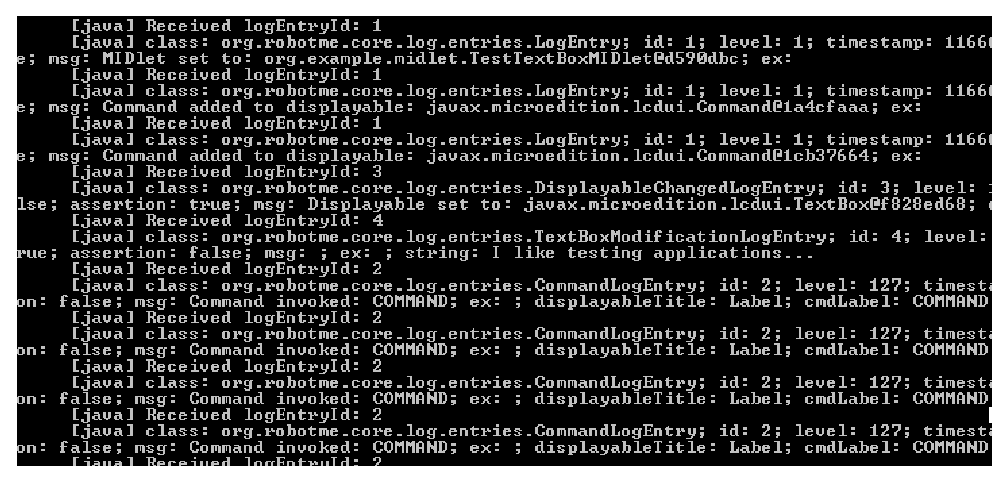
\includegraphics[height=4cm]{figures/2}}\fbox{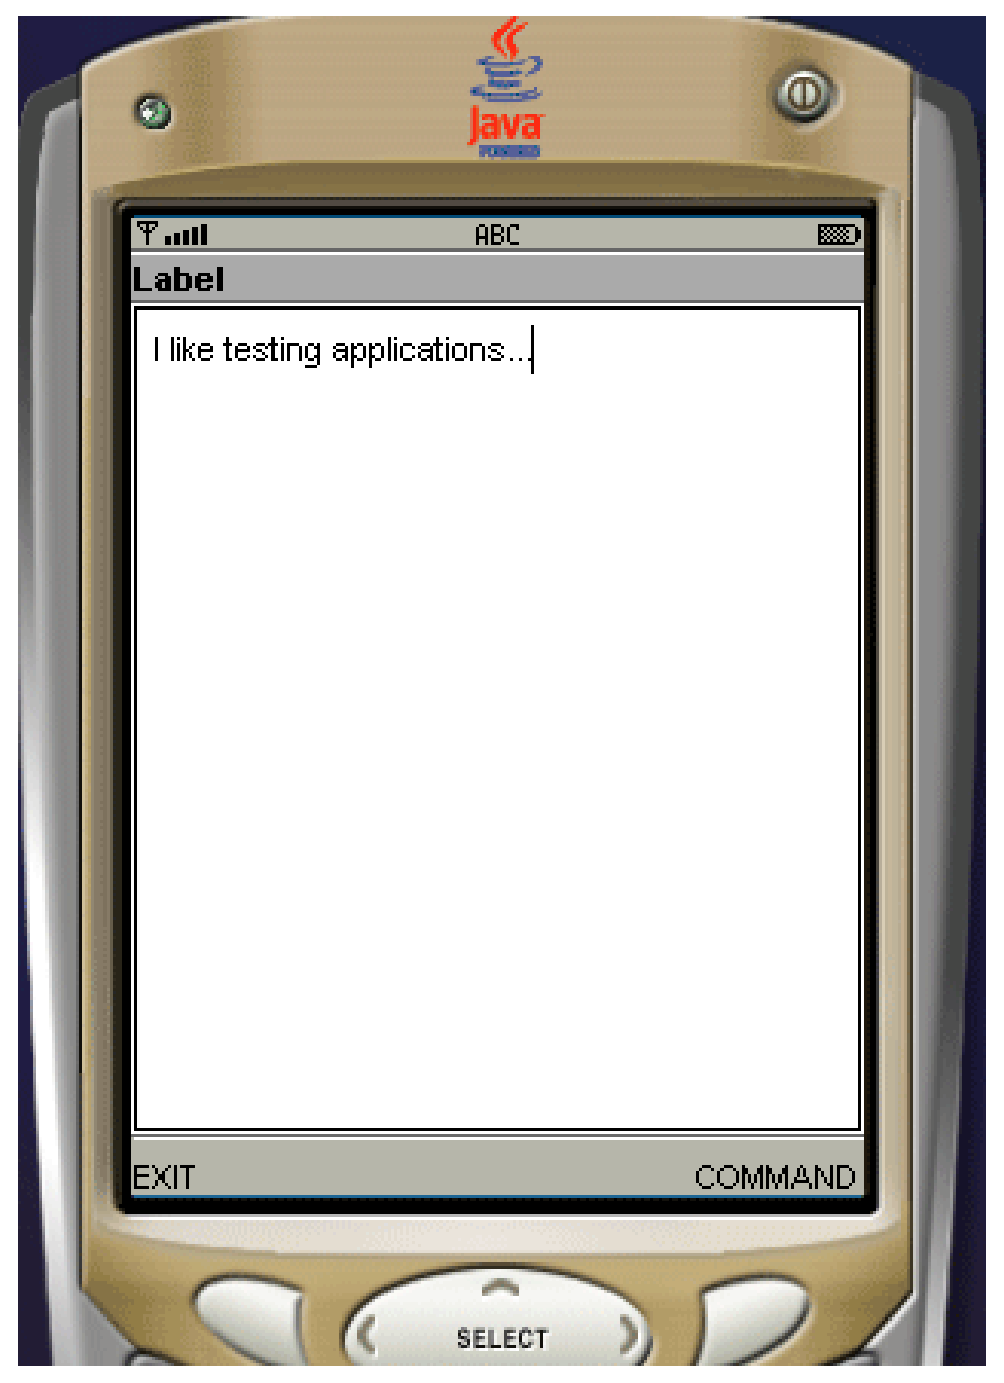
\includegraphics[height=4cm]{figures/1}}
\end{center}
\caption{Screenshots from test recording session. Server console (left) and emulator window (right).}%
\label{fig:session}
\end{figure}


%[To co uwazam na ta chwile bezpiecznie moznaby w tym punkie wstawic:
%- wyraznie powiedziec ze na razie mamy robota potrafiacego emulowac tylko czesc ze standardowych widgetow (?)
%- ze JAR z midletem wzrasta o ok 50 kb (obecnie jest to na poziomie 30 kb, ale jeszcze przeciez implementacji nie
%skonczylem, ale z drugiej strony te 30 to podaje bez obfuskacji)
%- ze czasowo (czas procesora) Robot polyk w znikomych ilosciach, praktycznie jest to pomijalne
%- oceniam (szacunkowo) ze Robot zabiera ok 30 kb RAMu
%- jest to prototyp, ktorego "produkcyjnie" nie testowalismy jeszcze, ale moze warto sie powolac na "rozmowy"
%i "zainteresowanie" ze strony przemyslu i powolac sie na NaviEpert, a byc moze tez na BreakPointGames (z tymi 
%ostatnimi nie rozmawialem jeszcze) ?
%]

%Testing schema that could be performed by NaviExpert thus improving quality of development product.

% [I may also ask guys from BreakPointGames company for permission of mentioning their as an example
% of world wide company that could gain real value from RobotME project --
% http://www.breakpointgames.com ]

\section{Future work}

As the framework we are describing is more a prototype for providing proof of concept and not a
production tool the first thing we will be focusing on is implementing the tool with full-fledged
support for all features of Java 2 Micro Edition compatible platforms. After achieving that we would
like to concentrate more on the following aspects:
%
\begin{itemize}
    \item Proposing flexible architecture of testing framework for simple addition of support for
    events that are outside of the scope of J2ME specification but are commonly used while
    developing mobile applications for certain vendors devices, for example vibra turning on or
    backlight switching support dedicated for one vendor, eg. Nokia.
    
	\item Allow sending recorded events to the server module not only through paid HTTP connection,
	but also through free serial cables and Bluetooth connections.
    
	\item To extremely simplify usage and lower start-up time for developers for employing the
	framework it is essential to integrate it with popular Integrated Development Environments like
	Eclipse or NetBeans. Many existing on the market continuous integration frameworks are
	exploiting build scripts written for ANT or Maven. It will be necessary to implement integration
	for all above tools in order to make our tool really powerful.
    
	\item As we are certain that our concept bring real benefits to mobile applications development
	industry we are thinking about extending it for other Java-based platforms for building mobile
	applications, like NTT DoCoMo Java or QUALCOMM BREW. They are not so worldwide popular as Java 2
	Micro Edition but in some parts of the globe are event superseding J2ME platforms and no testing
	frameworks for those platforms exists to our best knowledge as well. Such extensions will
	certainty need implementing another code injection techniques and other lifecycle manager for
	original mobile application but underlying concept for the testing framework will remain
	thesame.
\end{itemize}

%[W tym punkcie wspomniec o:
%- dokonczyc implementaje wszystkich standardowych widgetow
%- zaproponowac rozszerzalna architekture dla klas niestandardowych (jakies zdarzenia specyficzne dla konkretnych
%vendorow, np. zdarzenie wibratora)
%- rozszerzyc mozliwosc przekazywania eventow nie tylko poprzez GPRS (platny) ale takze poprzez serial i Bluetooth
%(bezplatne)
%- integracja z popularnymi narzedziami programistycznymi: ANT, Eclipse, NetBeans (wiele firm mobile'owych wlasnie
%NetBeans'a uzywa gdyz ma wbudowane wsparcie dla preprocessingu)
%- framework latwo mozna rozszerzyc na inne konkurencyjne dla J2ME platformy, takie jak japonska DoJA czy BREW (obie
%rowniez maja API Javowskie). Rozszerzenie sprowadzac sie bedzie do instrumentacji innym bytecodem i do napisania
%nowego core'a do zarzadzania cyklem zycia aplikacji na te platformy, natomiast koncepcja pozostanie niezmieniona.


\section{Summary and Conclusions}

We have presented a proof of concept demonstrating that fully-fledged capture-replay testing framework
is feasible in Java 2 Micro Edition environment. We have been working on the implementation of the above
ideas and have reported the initial feedback from the industry. While a number of issues still remain,
it seems that the core concept of implementing capture-replay tests for \jme{} development is feasible
and practical.

\raggedright
\bibliography{references}
\bibliographystyle{ieeetrans}

\end{document} 